\documentclass{article}
% Add this line for TeX Live
\usepackage{iftex}

% Encodings, page setup, paragraph formatting, font
\usepackage[top=0.9in, bottom=1in, left=1.5in, right=1.5in]{geometry}
\usepackage[icelandic]{babel}
\usepackage[T1]{fontenc}
\usepackage[sc]{mathpazo}
\usepackage[parfill]{parskip}
\usepackage{cancel}
\usepackage{comment}
% Tables and lists
\usepackage{booktabs,tabularx}
\usepackage{multirow}
\usepackage{enumerate}
\usepackage{adjustbox}
\usepackage{multicol}
\usepackage{enumitem}
\usepackage{xcolor}
% Math
\usepackage{amsmath, amsfonts, amssymb, amsthm}
% Graphics
\usepackage{graphicx}
\usepackage{forest}
\usepackage{tikz}
\usetikzlibrary{positioning, shapes, arrows.meta}
% Code environment
\usepackage{listingsutf8}
\definecolor{commentcolor}{RGB}{0, 128, 0} % Grænn
\definecolor{keywordcolor}{RGB}{0, 0, 255}   % Blár
\definecolor{stringcolor}{RGB}{163, 21, 21}      % Dökkrauður
\definecolor{numbercolor}{RGB}{128, 0, 128}      % Fjólublár
\definecolor{identifiercolor}{RGB}{0, 0, 0}      % Svartur

\lstset{
    language=C,
    basicstyle=\ttfamily,
    keywordstyle=\color{keywordcolor}\bfseries,
    commentstyle=\color{commentcolor},
    identifierstyle=\color{identifiercolor},
    stringstyle=\color{stringcolor},   
    showstringspaces=false,
    numbers=left,
    numberstyle=\tiny\color{gray},
    tabsize=2,
    breaklines=true,
    columns=fullflexible,
    keepspaces=true,
    inputencoding=utf8, 
    extendedchars=true,  
    literate=
        {á}{{\'a}}1
        {ð}{{\dh}}1
        {é}{{\'e}}1
        {í}{{\'i}}1
        {ó}{{\'o}}1
        {ú}{{\'u}}1
        {ý}{{\'y}}1
        {þ}{{\th}}1
        {æ}{{\ae}}1
        {ö}{{\"o}}1
        {Á}{{\'A}}1
        {Ð}{{\DH}}1
        {É}{{\'E}}1
        {Í}{{\'I}}1
        {Ó}{{\'O}}1
        {Ú}{{\'U}}1
        {Ý}{{\'Y}}1
        {Þ}{{\TH}}1
        {Æ}{{\AE}}1
        {Ö}{{\"O}}1,
}

% Restin af forskriftinni
\usepackage[pdftex,bookmarks=true,colorlinks=true,pdfauthor={Hafsteinn Einarsson},linkcolor=blue,urlcolor=blue]{hyperref}

% Hyphenation
\hyphenpenalty=5000
% Page and section numbering
\setcounter{secnumdepth}{-1} 
\pagenumbering{gobble}

\title{Tölvutækni og forritun Lokapróf}
\author{brj46 }
\date{Nóvember 2024}

\begin{document}

\maketitle

\vspace{5em}

\begin{center}
    
\includegraphics[scale = 0.2]{myndir/study.png}
\end{center}

\newpage

\section{Hvað þarf ég að kunna fyrir prófið?}

\begin{itemize}
    \item[$\square$] Bitavinnsla með heiltölur (signed og unsigned)
    \item[$\square$] Einfaldar fleytitölur
    \item[$\square$] Skrifa C kóða út frá smalamálskóða (reikniaðgerðir, styriskipanir, föll, bestun,...)
    \item[$\square$] Minnisyfirflæði (buffer overflow)
    \item[$\square$] Skyndiminni (Skipulag og notkun)
    \item[$\square$] Frabrigði, ferlar (fork, wait)
    \item[$\square$] Skipulag á sýndarminni
    \item[$\square$] Minnisúthlutun
\end{itemize}

\section {Hlutir til að setja á minnið}
\begin{itemize}
    \item \textbf{mov}: mov (move) flytur gildi á milli minnisstaða, t.d. \textbf{movl \%eax, \%ebx} flytur gildið í \textbf{\%eax} yfir í \textbf{\%ebx}
    \item \textbf{lea}: lea (load effective address) er notað til að reikna út minnisstaða og setja hana í register, t.d. \textbf{leaq (\%rbx, \%rcx, 4), \%rax} 
    reiknar út \textbf{rbx + (rcx * 4)} og setur í \textbf{\%rax}
    \item q: q stendur fyrir quadword sem er 64 bita gildi
    \item l: l stendur fyrir long sem er 32 bita gildi
    \item w: w stendur fyrir word sem er 16 bita gildi
    \item b: b stendur fyrir byte sem er 8 bita gildi
    \item \%rax: 64 bita register
    \item \%eax: 32 bita register
    \item \%ax: 16 bita register
    \item \%al: 8 bita register
    \item \textbf{Diane's Silk Dress Costs 89} (rdi, rsi, rdx, rcx, r8, r9)
    \item Formúla fyrir vistfang:
    \[\text{Vistfang} a[i][j] = \text{Upphafsvistfang} + ( i \times \text{fjöldi dalka} + j) \times \text{stærð staks}\]
\end{itemize}






\newpage

\section{Tekið frá Tuma}

\subsection{assembly}



\subsection{Uppbrot Gistis}

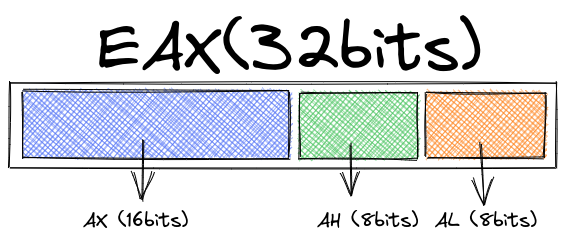
\includegraphics[scale = 0.8]{myndir/gistabrot.excalidraw.png}

\subsection{algengar skipanir}

\begin{tabularx}{\textwidth}{|l|l|X|}
\hline
    \textbf{skipun} & \textbf{argument} & \textbf{lýsing} \\ \hline
    mov & x, y & færir úr x yfir í y, sjá conditional move fyrir neðan\\ \hline 
    push & x & ýtir x á hlaða og eftir að hækka \text{\%ESP} um sizeof(x) bæti og sett þar inn \\ \hline
    pop & x & skilar síðasta gildi sem var sett á hlaðann inn í x \\ \hline
    lea & (x), y & lea, betur þekkt sem leaq er notað til að framkvæma reikning (x) og setja útkomu inn í y \\ \hline
    (x,y) & &skilar útkomu úr reikningi x + y \\ \hline
    0,(,x,y) & & skilar útkomu úr reikningi x * y \\ \hline
    (x,y,z) & & skilar útkomu úr reikningi x + y * z \\ \hline
    2(x, y, z) & & skilar útkomu úr reikningi (2 + (x + y * z)) \\ \hline
    sar & x, y & hliðrar y um x bita til hægri, basically heiltöludeiling með x\\ \hline
    sal & x, y & næstum eins og sar nema til vinstri, núna með margföldun með $2^x$ \\ \hline
    sub & x,y & dregur y frá x \\ \hline
    inc/dec & x & hækkar/lækkar gildi x um 1\\ \hline
\end{tabularx}

ath. \textbf{SHL} og \textbf{SAL} gera það sama en \textbf{SHR} virkar ekki með signed int eins og \textbf{SAR}

\subsection{Algeng mynstur}





\begin{tabularx}{\textwidth}{|l||X|}
\hline
 \textbf{ mynstur } &  \textbf{skýring} \\ \hline
    testl \%edi, \%edi & logical andað \textbf{edi} við \textbf{edi} þannig ef $edi <= 0$ er hægt að cmove eða jc í samræmi við það \\ \hline
    cmove $\$5$, \text{\%eax} & færðu 5 inn í eax ef z-flaggið er sett sem 1 þ.e. ef edi er tómt \\ \hline
    leal 0(\text{\%rdi, \%rdi, 4}) & margfaldar \text{\%rdi} með 5, $(x+4 *x)$ \\ \hline
\end{tabularx}
\newpage

\subsection{conditional codes}


þessir kóðar fara a endann á cmov skipunum þ.e. cmov-- í línu eftir að eitthvað er testað eins og í dæmi 

\begin{verbatim}
    testb   $7, %dl
    cmove   $1, %rax
\end{verbatim}

Þetta er pínu fucked dæmi því e flaggið í cmove stendur fyrir equal nema hvað við erum actually að athuga hvort útkomugildið sé 0, þ.e. að enginn af neðstu 3 bitunum sé 1, þá er gott að muna að e er jafngilt z

þessi koði færir 1 inn í \text{\%rax} ef neðstu þrír bitar \text{\%dl} eru ekki 111

\begin{tabular}{|c|c|}
\hline
     \textbf{cc}& \textbf{condition}  \\ \hline
    o  & overflow \\ \hline
    no & no overflow \\ \hline
    b, nae & below, not above or equal \\ \hline
    nb, ae & not below, above or equal \\ \hline
    e, z & equal(zero) \\ \hline
    ne, nz & not equal, (not zero) \\ \hline
    na, be & not above, below or equal \\ \hline
    a, nbe & above, not below or equal \\ \hline
    s & sign \\ \hline
    ns & no sign \\ \hline
    p & parity \\ \hline
    np & no parity \\\hline
    l, nge & less, not greater than or equal \\ \hline
    nl & not less, greater than or equal \\ \hline
    ng, le & not greater, less than or equal\\ \hline
    g, nle & greater, not less than or equal \\ \hline
\end{tabular}

\subsection{minnissvæði}


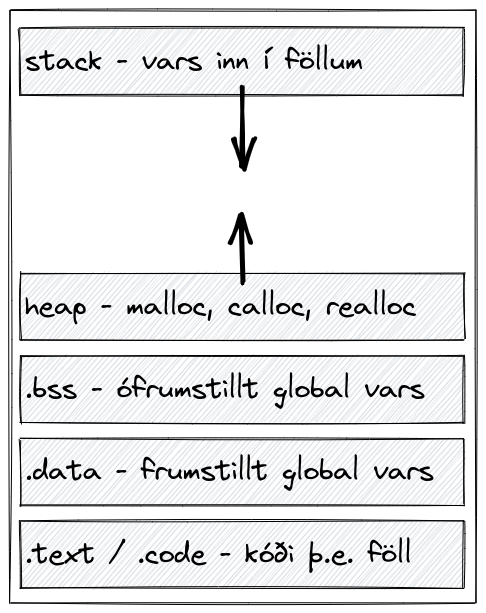
\includegraphics[scale = 0.4]{myndir/minni.excalidraw.png}

ath. global breytur sem eru skilgreindar sem 0 eða NULL eru líka í .bss
\newpage

\subsection{Sýndarminni}
\begin{itemize}
    \item sýndarvistföng: a bitar
    \item raunvistföng: b bitar
    \item síðustærð: c bæti
    \item TLB: d vítt, e sæti
    \item fjöldi mengha: f
\end{itemize}

fjöldi mengja er reiknað $\frac{e}{d} = f$

við erum með sýndarvistfang sem er 16 bitar sem skiptast í 4 mengi
þá er \textbf{VPN}$\frac{3}{4} \times 16$ bitar og \textbf{VPO} 4 bitar

\textbf{TBLT} og \textbf{TLBI} eru skipting á \textbf{VPN} og \textbf{TBLT} restin raunvistföngin eru jafn löng og \textbf{TLBT} og skipt niður í tvo hluta \textbf{PPN} og \textbf{PPO}, sem er jafn stór og \textbf{VPO}(í þessu tilfelli 4 bitar)

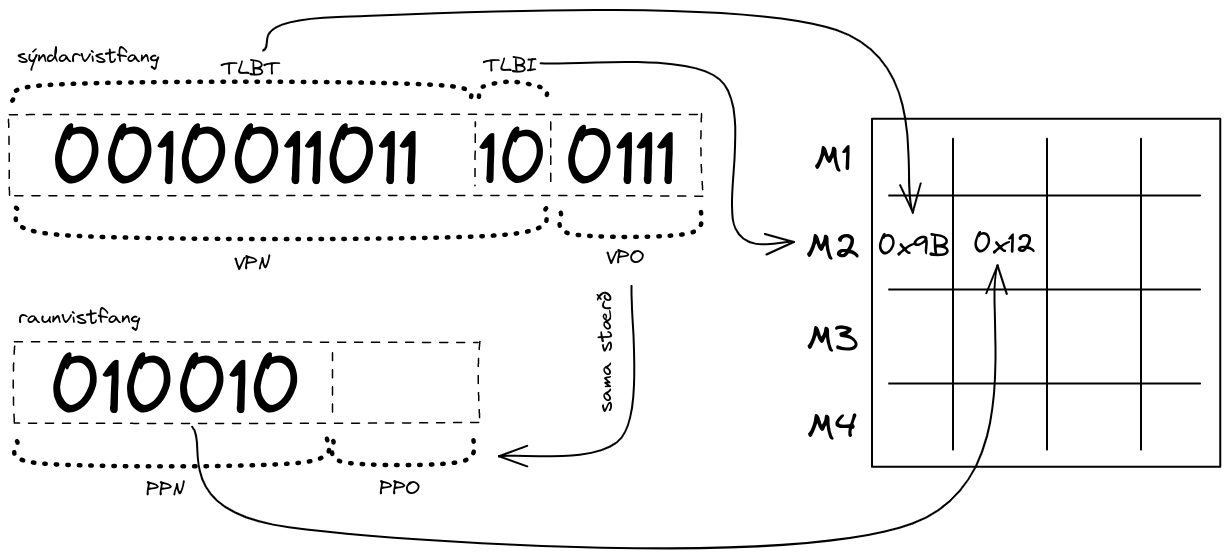
\includegraphics[scale = 0.2]{myndir/syndarminni.excalidraw.png}

annap dæmi, við erum með sýndarminni sem er 4kb að stærð, 4-vítt, E, og með 16 mengi, S, svo útfrá þessum tölum finnum við línustærð, B, með reikningnum $\frac{4096}{16 \times 4} = 64$ skiptum þessu nu upp fyrir 32-bita vistfang:

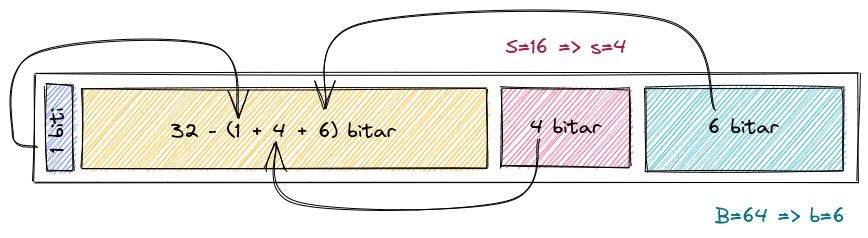
\includegraphics[scale = 0.3]{myndir/skipting.excalidraw.png}

\subsection{klukkutifsformúla}


$a + s \times r = m$
\begin{itemize}
    \item aðgangstími = a(tif)
    \item smellahlutfall = s(hlutfall)
    \item smellarefsing = r (tif)
    \item meðalaðgangstími = m (tif)
\end{itemize}

dæmi:
\begin{itemize}
    \item \text{97\%} smellahlutfall, $1 + 0.03 \times 100 = 4$
    \item \text{99\%} smellahlutfall, $1 + 0.01 \times 100 = 2$
\end{itemize}


\newpage
\section{Próf 2022 og mínar lausnir við því}
\subsection{1}
Í þessu dæmi ætlum við að nota unsigned long breytur til að tákna (allt að) 64
staka mengi (sets). Ef a er unsigned long breyta þá er stak i í menginu a ef biti i
($i = 0, \ldots 63$) er 1, annars er stak i ekki í menginu. Til dæmis væri mengið $\{0, 3\}$,
táknað með 64-bita bitastrengnum 00...01001. Athugið að bitarnir eru númeraðir frá
hægri til vinstri, svo stak 0 er í menginu, en stak 1 er ekki í menginu, stak 2 er ekki í
menginu, o.s.frv.

\subsubsection{a.}  Skrifið einnar línu fall (þ.e. bara ein \textbf{return} skipun) sem skilar sammengi
(union) tveggja slíkra mengja. Haus fallsins:
\textbf{unsigned long sammengi(unsigned long a, unsigned long b)}


\textbf{Svar}: 

\begin{lstlisting}
unsigned long sammengi(unsigned long a, unsigned long b){
    return a | b;
}
\end{lstlisting}



\subsubsection{b.}  Skrifið einnar línu fall sem skilar mengjamun (set difference) mengjanna a og b,
þ.e. öll stök sem eru í a, en ekki í b. Haus fallsins:
\textbf{unsigned long munur(unsigned long a, unsigned long b)}

\textbf{Svar}:

\begin{lstlisting}
unsigned long munur(unsigned long a, unsigned long b){
    return a & ~b;
}
\end{lstlisting}

\subsubsection{c.}  Athugið að í C er fastinn \textbf{1ul} (tölustafurinn \textbf{1} og bókstafirnir u og l) 64-bita
heiltalan 1 án formerkis. Hvaða mengi táknar segðin \textbf{($1ul << i$)}?

\textbf{Svar}:
Segðin \textbf{($1ul << i$)} táknar mengið sem inniheldur stakið i og engin önnur stök.

\subsubsection{d.}Skrifið einnar línu fall sem skilar því hvort stak i sé í menginu a. Skilagildið á
að vera 1 (\textit{satt}) ef i er í a, en 0 (\textit{ósatt}) annars. Þið megið gera ráð fyrir því að
gildið á i sé á bilinu 0 til 63. Haus fallsins:
\textbf{int stakI(unsigned long a, int i)}

\textbf{Svar}:
\begin{lstlisting}
    int stakI(unsigned long a, int i){
        return (a >> i) & 1;
    }
\end{lstlisting}

\newpage

\subsection{2}
Við höfum 10-bita fleytitölur sem fylgja IEEE staðlinum. Við vitum ekki
skiptingu þeirra í veldishluta (exp) og brothluta (frac), en það er einn formerkisbiti
fremst í þeim.

\subsubsection{a.}Hver er lágmarks bitafjöldi í brothluta fleytitölunnar til að hægt sé að tákna
töluna $3 \frac{9}{16}(=3.5625)$ nákvæmlega á þessu formi? Rökstyðjið svar ykkar með útreikningi.

\textbf{Svar}:
alright við vitum að í IEEE staðlinum erum við með fyrstu töluna sem segir til um + eða mínus næst kemur veldishlutinn og svo brothlutinn.

breytum 3.5625 í binary

\begin{align*}
    3.5625 &= 11.1001 \\
\end{align*}

setjum nú töluna í normað form ($1.f \times 2^n$) 
færum kommuna um einn stað til vinstri $1.11001 \times 2^1$ 
Veldisvísirinn er þá 1 og brothlutinn er 11001

svo Lágmarksbitafjöldi í brothlutanum er því 5 bitar


\subsubsection{b.}Hvert er bitagildið fyrir töluna $3 \frac{9}{16}(=3.5625)$ miðað við bitafjöldann fyrir brothlutann sem
þið funduð í a-lið (ef þið náðuð ekki að leysa a-liðinn megið þið gefa ykkur
raunhæft gildi bitafjöldanum fyrir brothlutann)? Sýnið útreikning á bitagildinu.


\textbf{Svar}:

þar sem við erum að vinna með 10 bita fleytitölur og við höfum að brothlutinn er 5 bitar
þá er veldishlutinn 4 bitar og formerkisbitinn er 1 biti

\begin{enumerate}
    \item Reiknum bias (skekkjustuðulinn)
    \[Bias = 2^{4-1} - 1 = 7\]
    \item Geymdur veldisvísir er þá
    \[GeymtE = E + Bias = 1 + 7 = 8\]
    8 í tvíundarkerfi er 1000
    \item setjum saman bitana:
    \begin{itemize}
        \item Formeki: 0 (jákvæð tala)
        \item Veldishlutinn: 1000
        \item Brothlutinn: 11001
    \end{itemize}

    \textbf{heildarbitaröðin og bitagildið er þá: 0 1000 11001}
\end{enumerate}



\subsubsection{c.} Segjum að í þessum 10-bita fleytitölum hefur verið ákveðið að nota einn bita
fyrir formerki, einn bita fyrir brothluta og restina af bitunum fyrir veldishlutann.
Er hægt að tákna staðlaðar tölur á þessu formi, og ef svo er, hver er þá \underline{stærsta
staðlaða talan} sem hægt er að tákna? Rökstyðjið svar ykkar.

\textbf{Svar}:
Já við getum táknað staðlaðar tölur á þessu formi 

\begin{itemize}
    \item Formerki: 1 biti
    \item Veldishlutinn: 8 bitar
    \item Brothlutinn: 1 biti
\end{itemize}


Reiknum Bias

\[2^{k-1} - 1= 2^{8-1} = 2^7 - 1 = 127\]

Hámarks veldistalan er þá $2^{8-1} - 1 = 127$

brothlutinn er 1 og við höfum gefinn 1 bita svo marktalan er 1.1 í binary sem í decimal er 1.5

stærsta staðlaða talan er því

\[1.5 \times 2^{127}\]

\subsubsection{d.} Nú hefur verið ákveðið að nota einn bita fyrir formerki, einn bita fyrir
veldishluta og restina af bitunum fyrir brothlutann. Er hægt að tákna staðlaðar
tölur á þessu formi, og ef svo er, hver er nú \underline{stærsta staðlaða talan} sem hægt er
að tákna? Rökstyðjið svar ykkar.

\textbf{Svar}:
Alright reynum þetta þá erum við með 

\begin{itemize}
    \item Formerki: 1 biti
    \item Veldishlutinn: 1 biti
    \item Brothlutinn: 8 bitar
\end{itemize}

reiknum bias

\[2^{k-1} - 1 = 2^{1-1} - 1 = 0\]

\textbf{Mögulegir veldisvísar eru þá: 0, 1}
\[E = 1 - 0 = 1\]

\textbf{Stærsta talan sem hægt er að tákna er þá:}
\[1.11111111_2 \times 2^1  = 1.(2^{1/2^1}+1/2^2+1/2^3+1/2^{\cdots}+2^8)=1.9960375 \times 2^1\]

\textbf{Stærsta staðlaða talan:}
\[1.9960375 \times 2^1 = 3.9921875\]

\newpage
\subsection{3}
Hér fyrir neðan er smalamálskóði fallsins fun:

\begin{verbatim}
    fun:
        movq    (%rdi), %rax
        jmp     .L2
    .L3:
        leaq    (%rax,%rax,2), %rax
        addq    %rax, %rax
        addq    $1, %rsi
    .L2:
        cmpq    %rdx, %rsi
        jl      .L3
        ret
\end{verbatim}


\subsubsection{a.} Hver er fjöldi vistfanga fallsins \textbf{fun} og hvert er tag hvers þeirra? Þið eigið að geta séð það út frá notkun gista í kóðanum hér að ofan. 
Rökstyðjið svarið með vísun í kóðann.


\textbf{Svar}:

Við höfum þrjár inntaksbreytur og eina staðværa breytu

\begin{itemize}
    \item \textbf{\%rdi} við sjáum að hér er \textbf{movq (rdi), rax} sem bendir til að þetta sé pointer á unsigned long gildi og fyrsta inntaksbreytan
    \item \textbf{\%rsi} Notað í samanburði \textbf{cmpq rdx, rsi} og síðan uppfærð með \textbf{addq \text{\$1}, rsi} þetta er önnur inntaksbreytan, líklega heiltala.
    \item \textbf{\%rdx} Notað í samanburði \textbf{cmpq rdx, rsi} þetta er þriðja inntaksbreytan og sennilega líka heiltala
    \item \textbf{\%rax} Notað til að geyma gildi sem er lesið úr mminni og síðan uppfært í lykkju.
\end{itemize}

því erum við með 4 vistföng

\begin{enumerate}
    \item \textbf{Bendir}: unsigned long * (í \text{\%rdi})
    \item \textbf{Heiltala s}: unsigned long (í \text{\%rsi})
    \item \textbf{Heiltala x}: unsigned long (í \text{\%rdx})
    \item \textbf{Staðvær heiltala rax}: unsigned long (í \text{\%rax})
\end{enumerate}


\subsubsection{b.}Skrifið jafngildan C kóða fyrir fallið \textbf{fun}. Þið megið velja breytunöfnin, eða
nefna þau eftir gistunum.

\textbf{Svar}:

\begin{lstlisting}
   unsigned long fun(unsigned long *ptr, unsigned long s, unsigned long x){
        unsigned long rax = *ptr;
        while(s < x){
            rax = 6 * rax;
            s = s + 1;
        }
        return rax;
    }
\end{lstlisting}


\subsubsection{c.} Smalamálskóðinn að ofan er úttak úr þýðandanum \textbf{gcc} með bestunarrofann
\textbf{-Og}. Ef notaður er bestunarrofinn \textbf{-O3} (sem er mesta mögulega bestun) fæst
kóðinn sem hér er fyrir neðan. Berið hann sama við fyrri kóðann og segið í
hvaða tilvikum \textbf{O3}-kóðinn gæti verið hraðvirkari.

\begin{verbatim}
    fun:
        movq    (%rdi), %rax
        cmpq    %rdx, %rsi
        jge     .L1
    .L3:
        leaq    (%rax,%rax,2), %rax
        addq    %rax, %rax
        addq    $1, %rsi
        cmpq    %rsi, %rdx
        jne     .L3
    .L1:
        ret

\end{verbatim}

\textbf{Svar}:
Byrjum á að skoða munin á milli þessara kóða :

við sjáum að í seinni kóðanum höfum við 
strax compare skipun í annari línu sem segir jge (jump greater or equal) sem þýðir að ef \textbf{rsi} er stærra eða jafnt og \textbf{rdx} þá er haldið áfram í \textbf{.L1} sem fer beint í return
þannig ef rsi er minna er rdx þá er farið í \textbf{.L3}

Næst fáum við leaq skipunina sem margfaldar rax með 3 og bætir í rax síðan er bætt rax við rax svo í raun er verið að gera
$6 \times rax$ síðan er 1 bætt við rsi og kannað hvort rsi sé orðið jafnt og rdx og ef ekki er farið aftur í \textbf{.L3} sem myndar lykkju.

ástæðan af hverju þetta er hraðvirkara er að það í seinna er færri hopp á milli. 



\newpage

\subsection{4}
Hér fyrir neðan er smalamálskóði fyrir endurkvæmt fall með hausinn:
\textbf{int rec(int n, int m)}:

\begin{verbatim}
    rec:
        cmpl    %esi, %edi  # lína 1
        jge     .L8         # lína 2
        movl    $0, %eax    # lína 3
        ret                 # lína 4
    .L8:
        subq    $8, %rsp    # lína 5
        addl    %esi, %esi  # lína 6
        subl    $2, %edi    # lína 7
        call    rec         # lína 8
        addl    $1, %eax    # lína 9
        addq    $8, %rsp    # lína 10
        ret                 # lína 11

\end{verbatim}

\subsubsection{a.} Sýnið jafngilt endurkvæmt C fall. Rökstyðjið einstakar skipanir út frá línum í
smalamálskóðanum.

\textbf{Svar}:

Byrjum á að skoða kóðann: 

\begin{itemize}
    \item lína 1 og 2: ef edi er stærra eða jafnt og esi þá er hoppað í \textbf{.L8}
    \item 3 og 4: ef edi er minna en esi þá er eax núllstillt og return skipun framkvæmd.
    \item lína 5: rsp er minnkað um 8
    \item lína 6: esi er tvöfaldast
    \item lína 7: edi er minnkað um 
    \item lína 8: kallað er á fallið rec
    \item lína 9: eax er hækkað um 1
    \item lína 10: rsp er hækkað um 8
    \item lína 11: return skipun
\end{itemize}

alright reynum að átta okkur á breytunum

\begin{itemize}
    \item edi: við höfum cmp(l) l tekur 32 bita sem þýðir að þetta er líklega heiltala 
    \item esi: við höfum cmp(l) sem þýðir að þetta er líklega heiltala
    \item eax: við höfum mov(l) skipun sem þýðir að þetta er líklega heiltala
    \item rsp: við höfum sub(q) q tekur 64 bita sem þýðir að þetta er líklega minnisvísir
\end{itemize}

\begin{lstlisting}
    int rec(int n, int m){
        if(n >= m){
            m = m + m;
            n = n - 2;
            int result = rec(n, m);
            return result + 1;
        }
        else{
            return 0;
        }
    }
\end{lstlisting}

\subsubsection{b.}Teiknið upp hlaðaramma (stack frame) \underline{fallsins \textbf{rec}} og merkið inn einstök
svæði í honum.

\textbf{Svar}:


\begin{center}
    \begin{tabular}{|c|}
        \hline
        \textbf{Endurkomuvistfang}\\ \hline
        \textbf{Ónotað pláss}\\ \hline
    \end{tabular}
\end{center}


\newpage

\subsection{5} Þrjár sjálfstæðar spurningar

\subsubsection{a.} Gefið er fylkið \textbf{short int a[6][10]}. Ef upphafsvistfang þess er 0, hvert
er þá vistfang staksins \textbf{a[3][4]}? Sýnið útreikning.

\textbf{Svar}:

notum víst þessa formúlu fyrir vistfang
\[ \text{Vistfang} a[i][j] = \text{Upphafsvistfang} + ( i \times \text{fjöldi dalka} + j) \times \text{stærð staks}\]
\begin{itemize}
    \item \textbf{Upphafsvistfang}: 0
    \item \textbf{fjöldi dalka}: 10
    \item \textbf{stærð staks}: 2 (short int) = 2 bæti
\end{itemize}

\textbf{Reiknum}:
\[ \text{Vistfang} a[3][4] = 0 + (3 \times 10 + 4) \times 2 = 0 + 34 \times 2 = 68\]

\textbf{Vistfang staksins a[3][4] er því 68}


\subsection{b.} Gefin er eftirfarandi færsla í C forriti:

\begin{verbatim}
    struct abcd {
        short int a[2];
        double b;
        char c;
        char *d;
};
\end{verbatim}

Rissið upp mynd af henni út frá uppröðunarkröfu (\textit{alignment requirements}) x86-
64. Hversu mörg bæti tekur færslan?

\textbf{Svar}:

Skoðum fyrst hvað hvert stak tekur af minni


\begin{itemize}
    \item Short int a[2]: 2 bæti
    \item Double b: 8 bæti
    \item Char c: 1 bæti
    \item Char *d: 8 bæti
\end{itemize}

\begin{center}
    \begin{tabularx}{\textwidth}{|l|l|X|}
        \hline
        \textbf{Offset} & \textbf{Biti} & \textbf{lýsing} \\ \hline
        0 & a[0] (2bæti) & fyrsta stak í a \\ \hline
        2 & a[1] (2bæti) & næsta stak í a \\ \hline
        4-7 & Padding (4 bæti) & Fylling til að halda réttri röð? \\ \hline
        8-15 & b (8 bæti) & double b \\ \hline
        16 & c (1 bæti) & char c \\ \hline
        17-23 & Padding (7 bæti) & Fylling til að halda réttri röð? \\ \hline
        24-31 & d (8 bæti) & char *d \\ \hline
    \end{tabularx}
\end{center}

\textbf{Færslan tekur því 32 bæti}

\subsection{c.} Skyndiminni er 2-vítt (\textit{2-way set associative}) með heildarstærðina 2048 (=211)
bæti og 16 (=24) bæta línur (þ.e. blokkir).

\textit{i.} Hvað hefur skyndiminnið mörg
mengi? 

\textbf{Svar}:
Til að finna Mengin skulum við nota formúluna

\[ \text{Fjöldi Mengi} = \frac{\text{Fjöldi lína}}{\text{Samstillingarstuðull}} \]

Til að finna heildarfjölda lína í skyndiminni er notað formúluna:

\[ \text{Fjöldi lína} = \frac{\text{Heildarstærð}}{\text{Línustærð}} = \frac{2048 \text{bæti}}{16 \text{bæti}} = 128 \text{línur}  \]

\textbf{Fjöldi mengja} er þá (samstillingarstuðulinn er 2 af því þetta er 2-vítt skyndiminni):

\[ \frac{128 \text{línur}}{2} = 64 \text{mengi} \]

\textit{ii.} Ef vistföng eru 16 bitar, hversu margir bitar eru þá notaðir fyrir
merkið (\textit{tag})?

\textbf{Svar}:

Til að finna fjölda merkisbita þurfum við að :

\begin{enumerate}
    \item finna fjölda bita fyrir block Offset
    \item finna fjölda bita fyrir set index
    \item Draga þessa bita frá heildarfjölda ita í vistfangi til að fá fjölda merkisbita.
\end{enumerate}

\textbf{Finnum fjölda bita fyrir block Offset}:

\[\textbf{Block offset} = \log_2(\text{Línustærð}) = \log_2(16) = 4 \text{bitar}\]

\textbf{Finnum fjölda bita fyrir set index}:

fjöldi mengja er 64 þannig að:

\[\textbf{Set index} = \log_2(\text{Fjöldi mengja}) = \log_2(64) = 6 \text{bitar}\]

\textbf{Fjöldi merkisbita}:

\[\textbf{Fjöldi merkisbita} = 16 - 4 - 6 = 6 \text{bitar}\]

\textbf{Merkisbitar eru því 6 bitar}

\newpage

\subsection{6} 

Hér fyrir neðan er forrit sem býr til ný ferli með fork-fallinu.

\begin{verbatim}
    void fall() {
        if (fork() != 0) {
            fork();
    	    printf("B\n");
        }
    }
    int main() {
        printf("A\n");
        fall();
        printf("C\n");
        exit(0);
    }

\end{verbatim}

\subsubsection{a.} Teiknið upp ferlarit (process graph) fyrir forritið og merkið inná það hvað
forritið prentar út á hverjum stað.

\textbf{Svar}:

Skoðum þetta forrit:

\begin{enumerate}
    \item lína 1: prentar út A
    \item lína 2: fallið fall er kallað
    \item lina 1 í falli: hér er kallað á fork (ferill P1) og ef það er ekki 0 þá er kallað á fork aftur
          hér heldur upprunalega ferlið P0 áfram þar sem Id hjá því er ekki 0 og því er kallað á fork aftur,
            það myndar nýtt ferli P2 Ferli.
    \item lína 3 í falli: Hér prenta ferli P0 og P2 út B en ekki P1 þar sem það stóðst ekki if skilyrðið þar sem fork() skilar 0.
    \item lína 4: prentar út C hér prenta allir 3 ferlarnir út C
    \item lína 5: hér er kallað á exit(0) í öllum ferlunum og því er forritið lokið.
\end{enumerate}

Skulum nú gera ferlarit:


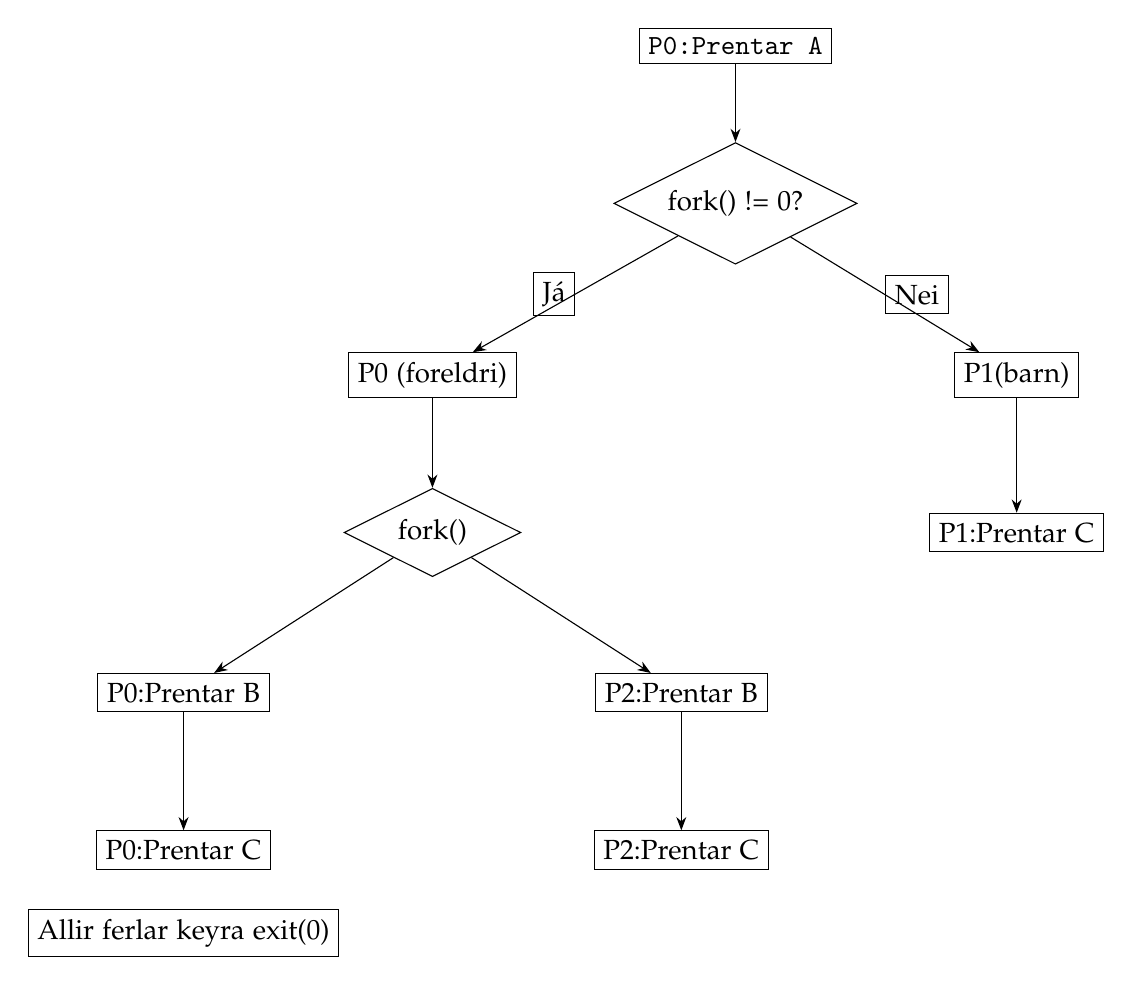
\begin{tikzpicture}[
    node distance=2cm,
    every node/.style={rectangle, draw, align=center},
    process/.style={rectangle, draw, align=center},
    decision/.style={diamond, draw, align=center, aspect=2},
    >=Stealth
]


\node[process] (start) {\texttt{P0:Prentar A}};
\node[decision, below of=start](fork1){fork() != 0?};
\node[process, below left=1.5cm and 2cm of fork1](P0){P0 (foreldri)};
\node[process, below right=1.5cm and 2cm of fork1](P1){P1(barn)};
\node[decision, below of=P0](fork2){fork()};
\node[process, below left=1.5cm and 1.5cm of fork2](P0_B){P0:\text{Prentar B}};
\node[process, below right=1.5cm and 1.5cm of fork2](P2){P2:\text{Prentar B}};
\node[process, below of=P1] (P1_C){P1:\text{Prentar C}};
\node[process, below of=P0_B] (P0_C){P0:\text{Prentar C}};
\node[process, below of=P2] (P2_C){P2:\text{Prentar C}};

\draw[->] (start) -- (fork1);
\draw[->] (fork1) -- node[left]{Já} (P0);
\draw[->] (fork1) -- node[right]{Nei}(P1);
\draw[->] (P0) -- (fork2);
\draw[->] (fork2) -- (P0_B);
\draw[->] (fork2) -- (P2);
\draw[->] (P1) -- (P1_C);
\draw[->] (P0_B) -- (P0_C);
\draw[->] (P2) -- (P2_C);

\node[below=0.5cm of P0_C] (exit0) {Allir ferlar keyra exit(0)};

\end{tikzpicture}


\subsection{b.} Sýnið þrjár ólíkar mögulegar útprentanir sem forritið getur gert.

\textbf{Svar}:

Þar sem allir ferlarnir keyra á sama tíma en bara eftir að er kallað á þá þannig mögulegar útkomur eru:
\begin{itemize}
    \item A C B C B C
    \item A B B C C C
    \item A B C B C C
\end{itemize}


\subsection{c.} Hversu mörg ferli munu framkvæma skipunina "exit(0)" í main-fallinu?
Rökstyðjið svarið!

\textbf{Svar}:

Allir ferlarnir munu framkvæma skipunina exit(0) þar sem það er kallað á hana í main fallinu og því munu allir ferlarnir loka.

\newpage

\section{Próf 2021 - Og mín Heiðarleg tilraun á að leysa það}

\subsection{1.} Í þessu dæmi höfum við 6-bita orðið \textbf{010011}. Það er hægt að túlka það á þrjá vegu
sem gildi: \textit{i}. 6-bita heiltala án formerkis (unsigned), \textit{ii}. 6-bita tvíandhverfu heiltala
(signed) og \textit{iii}. 6-bita fleytitala (floating point) með 1 formerkisbita, 3 veldisbita og 2
brotbita.

\subsubsection{a.}Túlkið orðið 010011 sem gildi á þessa þrjá vegu. Sýnið útreikning (sérstaklega
í fleytitölunni).

\textbf{Svar}:

\begin{itemize}
    \item \textbf{6-bita heiltala án formerkis}: reiknum þá $2^0+2^1+2^4 = 19 $ 
    \item \textbf{6-bita tvíandhverfu heiltala}: Reiknum þá sem signed Þar sem það er 0 fremst þá er þetta jákvæð tala og skilar sama svari 
                                                 og án formerkis þannig $2^0+2^1+2^4 = 19$ 
    \item \textbf{6-bita fleytitala}: sem 6 bita fleyti tala með 1 formerkisbita og 3 veldisbita og 2 brotbita þá höfum við 0 fyrir jákvæða tölu
                                      100 sem veldisbita og 11 sem brotbita. við þurfum fyrst að reikna raunverulegan veldisvisi (\textbf{E})
                                      fyrir það þurfum við fyrst að reikna skekkjustuðulinn sem er reiknaður :
                                      \[\text{Bias} = 2^{k-1}-1= 2^{3\text{(bitar)}-1}-1 = 2^2-1 = 4 - 1= 3\]
                                      Reiknum nú \[E = \text{bitagildið þ.e.a.s 100 = 4} - \text{Bias} = 4-1 \]
                                      Svo raunverulegi veldisvísirinn er 1 semsagt $2^1$
                                      nú finnum við brothlutann $11$ við vitum að það er gefinn 1 á undan brothluta svo við fáum $1.11$ 
                                      til að reikna brothluta gerum við $1.(2^{1/2}+2^{1/4}) = 1.75$
                                      Setjum þetta nú saman \[ + 1.75 \times 2^1 = 3.5\]                                
\end{itemize}

\subsubsection{b.}Þið megið breyta einum bita í orðinu að ofan og viljið fá sem hæst gildi (þ.e.
sem næst $+\infty$). Sýnið og rökstyðjið í hverju tilviki hvaða bita þið mynduð
breyta til að hámarka gildið. Það geta verið ólíkir bitar í hverri túlkun

\textbf{svar}: 
\begin{itemize}
    \item[a.] í unsigned þá myndum við bæta 1 fremst þar sem hægt veri svo $(1)10011 = 1+2+16+32=51 $ 
    \item[b.] í signed þá má fremsti ekki vera 1 þar sem þá er talan í mínus svo $01(1)011 = 1+2+8+16 = 27$
    \item[c.] hér myndum við vilja bæta á veldisvísinn svo þá væri talan $0 110 11$ 
                Reiknum skekkjuna $\text{bias} = 2^{3-1} -1 = 2^2 -1 = 4-1 = 3$
                Reiknum Raunverulegann veldisvísi $e - \text{bias} =  6 - 3 = 3$
                Svo talan yrði $1.75 \times 2^3 = 1.75 \times 8 = 14$ 
\end{itemize}

\subsubsection{c.} Hvaða einum bita ætti að breyta til að lágmarka gildið (þ.e. komast sem næst
$-\infty$) í hverri túlkun? Rökstyðjið hvert tilvik

\textbf{svar}: 
\begin{itemize}
    \item[a.] í unsigned þá myndum við taka 0 fremst þar sem hægt veri svo $000011 = 1+2 = 3 $ 
    \item[b.] í signed þá setjum við fremsta sem 1 þar sem þá er talan í mínus svo $(1)10011 = -32 + 16+2+1  = -13$
    \item[c.] hér myndum við vilja setja formerkisbitann sem 1 til að fá töluna í mínus svo  þá væri talan $1 100 11$ 
                Reiknum skekkjuna $\text{bias} = 2^{3-1} -1 = 2^2 -1 = 4-1 = 3$
                Reiknum Raunverulegann veldisvísi $e - \text{bias} =  4 - 3 = 1$
                Svo talan yrði $-1.75 \times 2^1 = -1.75 \times 2 = -3.5$ 
\end{itemize}
\newpage 

\subsection{2}Hér fyrir neðan er x86-64 smalamálsútgáfa af endurkvæma fallinu func.

\begin{center}
    \begin{verbatim}
        func:
            cmpl    $1, %edi
            jle     .L3
            pushq   %rbx
            leal    (%rdi,%rdi,2), %ebx
            leal    3(%rdi), %edx
            testl   %edi, %edi
            cmovns  %edi, %edx
            sarl    $2, %edx
            movl    %edx, %edi
            call    func   
            addl    %ebx, %eax
            popq    %rbx
            ret 
        .L3:
            movl    $1, %eax
            ret
    \end{verbatim}
\end{center}

\subsubsection{a.}Skrifið jafngilda C útgáfu af þessu falli. Til að hjálpa ykkur við það er hér fyrir
neðan beinagrind af fallinu sem þið getið fyllt inn í. Rökstyðjið sérstaklega
hvaða smalamálsskipanir standa á bakvið þann kóða sem þið setjið inn.

\begin{verbatim}
    int func(int n) {
        if ( _____ )
            return _____;
       return _____ + func( _____ );
    }
\end{verbatim}

\textbf{svar}: 
Alright skoðum hvað línurnar gera
\begin{itemize}
    \item Lína 1: berum edi við 1
    \item Lína 2: ef edi er 1 eða minna þá er hoppað í \textbf{.L3}
    \item Lína 3: ýtt rbx á hlaðann
    \item Lína 4: rdi sinnum 3 sett í ebx
    \item Lína 5: 3 + rdi sett í edx
    \item Lína 6: skoðar hvort edi sé neikvætt eða ekki
    \item Lína 7: ef edi er ekki neikvætt þá er edx = n annars er edx = n+3
    \item Lína 8: shift arithmetically right eða $ edi >> 2 $ sem deilir með 4
    \item Lína 9: setur edi í edx
    \item Lína 10: callað á func
    \item Lína 11: ebx bætt við eax þar sem ebx er 3 * n þannig $eax = eax + ebx$
    \item Lína 12: rbx poppað af hlaðanum endurheimt gildi úr kösinni
    \item Lína 13: return skipun
    \item Lína 14: sett eax sem 1
    \item lína 15: return skipun
\end{itemize}

Reynum nú að setja þetta í c fall:

\begin{lstlisting}
int func(int n){
    if(n >=1)
        return 1;
    return (3*n) + func((n >= 0 ? n : n+3) / 4);
}
\end{lstlisting}

\subsubsection{b.}Teiknið upp hlaðaramma (\textit{stack frame}) fyrir fallið. Sýnið stöðuna þegar þrjú
endurkvæm köll hafa orðið. Tilgreinið einstaka hluta hvers hlaðaramma.

\begin{center}
    
\end{center}

\newpage
\subsection{3}
Hér fyrir neðan er C fall sem afritar eitt stak á milli tveggja tvívíðra fylkja. Fylkin
eru víðvær og er fylkið a af stærðinni \textbf{MxN}, en \textbf{b} er af stærðinni \textbf{NxM}. Þið viti ekki
gildin á \textbf{M} eða \textbf{N}, en eigið að geta fundið þau útfrá smalamálskóðanum fyrir fallið sem
einnig er gefinn.

\begin{verbatim}
    long int a[M][N];
    long int b[N][M];

    void afrit( int i, int j ) {
        a[i][j] = b[j][i];  
    }
\end{verbatim}
\begin{verbatim}
    afrit:
        movslq      %edi, %rdi
        movslq      %esi, %rsi
        leaq        0(,%rsi,8), %rax
        subq        %rsi, %rax
        addq        %rdi, %rax
        movq        b(,%rax,8), %rdx
        leaq        (%rdi,%rdi,4), %rax
        leaq        (%rdi,%rax,2), %rax
        addq        %rax, %rsi
        movq        %rdx, a(,%rsi,8)
        ret
\end{verbatim}

\subsubsection{a.}Hver eru gildin á \textbf{M} og \textbf{N}? Rökstyðjið svörin út frá skipununum í
smalamálskóðanum.


\textbf{svar}: ef við fylgjum diane's silk dress cost 89 þá sjáum við að 
edi er þar að leiðandi i og esi er þá j. 

skoðum nú línurnar
\begin{itemize}
    \item Lína 1: setur 32 bita innihald edi í 64 bita innihald rdi þannig rdi fær i
    \item Lína 2: setur 32 bita innihald esi í 64 bita rsi þannig rsi fær j
    \item Lína 3: rsi * 8 sett í rax þannig rax er jafnt og 8 * j
    \item Lina 4: rax - rsi þannig rax = 7 * j
    \item Lína 5: rax + rdi þannig rax = 7 * j + i
    \item Lína 6: b + 8 * rax sett í rdx þ.e.a.s (7 * j + i)
    \item Lína 7: rdi * 5 sett í rax
    \item Lína 8: rax * 2 + rdi sett í rax ( þannig 11 * rdi sett í rax)
    \item Lína 9: rax = rax + rdi (rsi = j + 11 * i)
    \item Lína 10: skrifar gildi úr rdx á vistfanginu a + rsi * 8
    \item Lina 11: return
\end{itemize}

\textbf{út frá þessu notum við}:


\[\textbf{Visfang} = b + ( j \times M + i) \times 8\]

Út frá smalarmálskóðanum fyrir b þá fáum við
\[ \text{Offset fyrir b[j][i]} = 7j + i\]

jafnsetjum:
\[j \times M + i = 7j + i\]

Einangrum M

\[M = 7\]

Gerum nú fyrir a:

\[ \text{Vistfang} = a  + (i \times N \times j) \times 8\]

út frá smalamálinu fáum við

\[ \text{offset fyrir a[i][j]} = 11i +j\]

jafnsetjum:

\[ i \times N \times j = 11i +j\]

einangrum N
\[ N = 11\]

svo gildin eru 

$M = 7$
$N = 11$




\subsubsection{b.}:Ef bæði fylkin hefðu verið skilgreind með stærðina \textbf{MxN} hefði þá verið hægt að
finna gildið á bæði \textbf{M} og \textbf{N} (eða annað hvort þeirra) út frá smalamálskóðanum?
Rökstyðjið svar ykkar.

\textbf{Svar:} nei ekki hægt en vá hvað ég nenni því ekki að fara út í af hverju

\newpage
\subsection{4} Hér fyrir neðan eru súlurit fyrir lestrarafköst tveggja ólíkra tölva. Gildin eru
fengin úr minnisfjalli (\textit{memory mountain}) fyrir tölvurnar. Það er tekinn skurður í
gegnum minnisfjallið við skrefstærð (\textit{stride}) 8, svipað og gert var í einu heimadæmi í
námskeiðinu. Í súluritinu er x-ásinn stærð vinnumengisins (\textit{working set}), þ.e. stærð
fylkjanna sem unnið er með, og y-ásinn sýnir lestrarafköst í MB/sek. Dökku súlurnar
sýna afköst tölvu A, en ljósu súlurnar sýna afköst tölvu B. Notið súluritin til að svara
eftirfarandi spurningum:


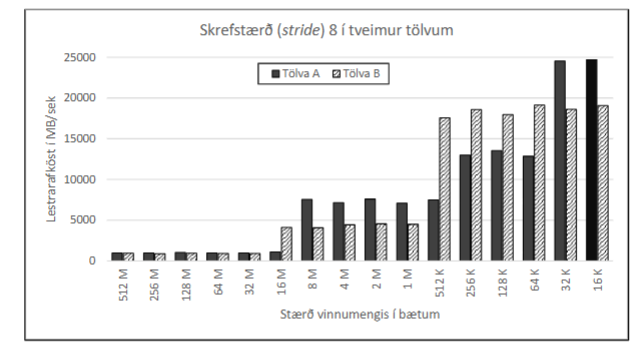
\includegraphics[scale = 0.7]{myndir/prof2021d4.png}


\subsubsection{a.}Hversu mörg lög (\textit{levels}) af skyndiminni eru í tölvu A og hversu stórt má áætla
að hvert þeirra sé? Rökstyðjið svarið!

\subsubsection{b.}Hversu mörg lög (\textit{levels}) af skyndiminni eru í tölvu B og hversu stórt má áætla
að hvert þeirra sé? Rökstyðjið svarið!

\subsubsection{c.}Tiltekið forrit notar tætitöflu (\textit{hash table}) nokkuð mikið. Taflan hefur 50.000
stök, sem hvert er 8 bæti að stærð. Hvor tölvan væri hagkvæmari fyrir þetta
forrit? Rökstyðjið.

\subsubsection{d.}Breytist svar ykkar við c-lið ef tætitaflan stækkar, t.d. tvöfaldast eða þrefaldast?
Rökstyðjið.

\subsubsection{e.}Er hægt að segja eitthvað um uppsetningu skyndiminnanna (þ.e. línustærð, vídd,
eða fjölda mengja) í tölvunum tveimur út frá þessum súluritum? Rökstyðjið.

\section{Vika 1}
\large{\textbf{Kynning, Linux, C}}


\section{Vika 2}
\large{\textbf{C, Bendar, minni, notkun}}


\section{Vika 3}
\large{\textbf{Upplýsingar sem bitar, heiltölur}}


\section{Vika 4}
\large{\textbf{Bætaröð, fleytitölur}}


\section{Vika 5}
\large{\textbf{Skipulag örgjava, smalamálsforritun}}


\section{Vika6}
\large{\textbf{Stýriskipanir og stef í smalamáli}}


\section{Vika 7}
\large{\textbf{Gögn og yfirflæði minnis}}


\section{Vika 8}
\large{\textbf{Bestun smalamálskóða}}


\section{Vika 9}
\large{\textbf{Minnisstigveldi, skyndiminni}}


\section{Vika 10}
\large{\textbf{Tenging, keyrsluskrár, forritasöfn}}


\section{Vika 11}
\large{\textbf{Frábrigði, ferlastýring}}

\section{Vika 12}
\large{\textbf{Sýndarminni}}

\section{Vika 13}
\large{\textbf{Minnisúthlutun, ruslasöfnun, minnisvillur}}


\section{Vika 14}
\large{\textbf{Samantekt}}


\end{document}
